% A skeleton file for producing Computer Engineering reports
% https://kgcoe-git.rit.edu/jgm6496/KGCOEReport_template

\documentclass[CMPE]{KGCOEReport}

% The following should be changed to represent your personal information
\newcommand{\classCode}{CMPE 160}  % 4 char code with number
\newcommand{\name}{Andrei Tumbar}
\newcommand{\LabSectionNum}{4}
\newcommand{\LabInstructor}{Mr.\ Byers}	% The slash is to tell LaTeX that the period is between words
												% not sentences so it spaces correctly. It won't appear in the
												% final pdf
\newcommand{\TAs}{Sam Myers \\ Kobe Balin \\ Georgi Thomas}
\newcommand{\LectureSectionNum}{1}
\newcommand{\LectureInstructor}{Mr.\ Cliver}
\newcommand{\exerciseNumber}{5}
\newcommand{\exerciseDescription}{Combinational Logic Circuit Design Using Karnaugh Map Simplification}
\newcommand{\dateDone}{February 13th}
\newcommand{\dateSubmitted}{February 20th}

\graphicspath{{./lab5_media/}}

\usepackage{circuitikz}
\usepackage{tikz}
\usepackage{multirow}
\usepackage{titlesec}
\usepackage{float}
\usepackage{pgfplots, pgfplotstable}
\usepackage{lmodern}
\usepackage{siunitx}
\usepackage{subcaption}

\usepackage{kmap}
\usepackage[T1]{fontenc}

\usepackage{amsmath}

\ctikzset{bipoles/not port/circle width=.4}
\ctikzset{tripoles/american and port/width=0.8}

\DeclareFontFamily{U}{mathx}{\hyphenchar\font45}
\DeclareFontShape{U}{mathx}{m}{n}{ <-> mathx10 }{}
\DeclareSymbolFont{mathx}{U}{mathx}{m}{n}
\DeclareFontSubstitution{U}{mathx}{m}{n}
\DeclareMathAccent{\widebar}{\mathalpha}{mathx}{"73}

\makeatletter
\newcommand{\cwidebar}[2][0]{{\mathpalette\@cwidebar{{#1}{#2}}}}
\newcommand{\@cwidebar}[2]{\@cwideb@r{#1}#2}
\newcommand{\@cwideb@r}[3]{%
  \sbox\z@{$\m@th#1\mkern-#2mu#3\mkern#2mu$}%
  \widebar{\box\z@}%
}
\makeatother

\begin{document}
\maketitle

\section*{Abstract}
In this laboratory exercise, an arbitrary function was implemented using a simplified Karnaugh map. A product of sums and a sums of product expression was generated. Both circuits were designed in Quartus II and then simulated in Modelsim. A forces file was initially used to control input pins, however, the test bench provided on MyCourses proved to be a more effient way to test the circuit. The cost of each circuit was evaluated. The cheap circuit was implemented a breadboard. The function was a four-input, one-output function described using min-term notation. The exercise was successful when implementing the circuit on a breadboard as well in the Modelsim simulation.

\section*{Design Methodology}

A function provided in equation \ref{eq:func} is a min-term representation of $F$.

\begin{equation}
\label{eq:func}
F = {\sum}_{ABCD} (0,2,3,4,6,7,13,14,15)
\end{equation}

Every number above shows in the input combinations that would result in a 1 in binary. The 4-bit input is represented by $A$, $B$, $C$, and $D$ in that order.

\subsection*{Karnaugh Maps}

Two Karnaugh Maps were created to implement the function using max-term and min-terms. The sum-of-products (min-terms) and product-of-sums (max-terms) expressions were found below.

\begin{figure}[h!]
	\begin{subfigure}{.5\textwidth}
		\centering
		\begin{Karnaugh}
				\contingut{1,0,1,1,
						   1,0,1,1,
						   0,0,0,0,
						   0,1,1,1}
		   \implicantcostats{0}{6}{red}
		   \implicant{3}{6}{blue}
		   \implicant{7}{14}{green}
		   \implicant{13}{15}{yellow}
		\end{Karnaugh}
		\caption{Min-terms K-Map}
		\label{fig:sop}
	\end{subfigure}
	\begin{subfigure}{.5\textwidth}
		\centering
		\begin{Karnaugh}
				\contingut{1,0,1,1,
						   1,0,1,1,
						   0,0,0,0,
						   0,1,1,1}
		   \implicant{8}{10}{blue}
		   \implicant{12}{8}{red}
		   \implicant{1}{5}{green}
		\end{Karnaugh}
		\caption{Max-terms K-Map}
		\label{fig:pos}
	\end{subfigure}
	
	\caption{K-Maps for both POS and SOP functions}
	\label{fig:kmap}
\end{figure}

The groups in Figure \ref{fig:kmap} were written as a sum-of-products (SOP) and a product-of-sums (POS). Figure \ref{fig:sop} shows 4 groupings and therefore 4 terms were generated. Figure \ref{fig:pos} however, shows 3 groupings.

\subsection*{Reduced Expressions}

An expression can be extracted from each expression. This results in a boolean expression in POS or SOP form.

\begin{equation}
\label{eq:sop}
F_{SOP} = \widebar{A}\widebar{D} + ABD + \widebar{A}C + BC
\end{equation}

\begin{equation}
\label{eq:pos}
F_{POS} = (\widebar{A} + B)(\widebar{A} + C + D)(A + C + \widebar{D})
\end{equation}

The SOP (Eq. \ref{eq:sop}) and POS (Eq. \ref{eq:pos}) expressions above can be implemented using a circuit with AOI logic.

\begin{figure}[htbp]
	\centering
	\begin{circuitikz}[scale = 0.8, transform shape]
	
	\coordinate (TOP) at (0,12);
	
	\draw (TOP) to[short, l=A, o-] ++(1,0) to[short, -*] ++(1,0) coordinate(A);
	\draw (TOP) ++(0,-1) to[short, l=B, o-] ++(1,0) to[short, -*] ++(2.5,0) coordinate(B);
	\draw (TOP) ++(0,-2) to[short, l=C, o-] ++(1,0) to[short, -*] ++(4,0) coordinate(C);
	\draw (TOP) ++(0,-3) to[short, l=D, o-] ++(1,0) to[short, -*] ++(5.5,0) coordinate(D);
	
	\draw (A) ++(0.5,0) node (anot) [not port, scale=.5]{};
	%\draw (B) ++(0.5,0) node (bnot) [not port, scale=.5]{};
	%\draw (C) ++(0.5,0) node (cnot) [not port, scale=.5]{};
	\draw (D) ++(0.5,0) node (dnot) [not port, scale=.5]{};
	
	\draw (A) -- (anot.in)
		  %(B) -- (bnot.in)
		  %(C) -- (cnot.in)
		  (D) -- (dnot.in);
	
	\draw (anot.out) |- ++(-0.4,-0.4) coordinate(!A);
	%\draw (bnot.out) |- ++(-0.4,-0.4) coordinate(!B);
	%\draw (cnot.out) |- ++(-0.4,-0.4) coordinate(!C);
	\draw (dnot.out) |- ++(-0.4,-0.4) coordinate(!D);
	
	\coordinate (SOP_TOP) at (10,7);
	
	\draw (SOP_TOP)              node (sop_t1) [and port, scale=0.7]{};
	
	\draw (SOP_TOP) ++(0,-1.5)   node (sop_t2_1) [and port, scale=0.7]{};
	\draw (SOP_TOP) ++(1.5,-2)   node (sop_t2_2) [and port, scale=0.7]{};
	
	\draw (SOP_TOP) ++(0,-3)     node (sop_t3)   [and port, scale=0.7]{};
	
	\draw (SOP_TOP) ++(0,-4.5)   node (sop_t4)   [and port, scale=0.7]{};
	
	\draw (SOP_TOP) ++(3,-0.5)     node (sop_c1) [or port, scale=0.7]{};
	\draw (SOP_TOP) ++(4.75,-2.25) node (sop_c2) [or port, scale=0.7]{};
	\draw (SOP_TOP) ++(2,-3.75)  node (sop_c3) [or port, scale=0.7]{};
	
	\draw (!A) |- node[circ,midway]{} (sop_t1.in 1)
		  (!D) |- node[circ,midway]{} (sop_t1.in 2)
		  ;
	
	\draw (A) |- node[circ,midway]{} (sop_t2_1.in 1)
		  (B) |- node[circ,midway]{} (sop_t2_1.in 2)
		  (D) |- node[circ,midway]{} (sop_t2_2.in 2)
		  
		  (sop_t2_1.out) -- ++(0.35, 0) |- (sop_t2_2.in 1)
		  ;
	
	\draw (!A) |- node[circ,midway]{} (sop_t3.in 1)
		  (C)  |- node[circ,midway]{} (sop_t3.in 2)
		  ;
		  
	\draw (B)  |- node[circ,midway]{} (sop_t4.in 1)
		  (C)  |- node[circ,midway]{} (sop_t4.in 2)
		  ;
	
	\draw (sop_t1.out) -- ++(1.5,0) |- (sop_c1.in 1)
		  (sop_t2_2.out) -- ++(0.25,0) |- (sop_c1.in 2);
	
	\draw (sop_t3.out) -- ++(0.25,0) |- (sop_c3.in 1)
		  (sop_t4.out) -- ++(0.25,0) |- (sop_c3.in 2);
	
	\draw (sop_c1.out) -- ++(0.25,0) |- (sop_c2.in 1)
		  (sop_c3.out) -- ++(1.25,0)  |- (sop_c2.in 2);
	
	\draw (sop_c2.out) to[short, l=$F_{SOP}$, -o] ++(1.75,0);
	
	
	\coordinate (POS_TOP) at (10,-1);
	
	\draw (POS_TOP)            node (pos_t1)   [or port, scale=0.7]{};
	
	\draw (POS_TOP) ++(0,-1.5) node (pos_t2_1) [or port, scale=0.7]{};
	\draw (POS_TOP) ++(2,-2)   node (pos_t2_2) [or port, scale=0.7]{};
	
	\draw (POS_TOP) ++(0,-3)   node (pos_t3_1) [or port, scale=0.7]{};
	\draw (POS_TOP) ++(2,-3.5) node (pos_t3_2) [or port, scale=0.7]{};
	
	
	\draw (POS_TOP) ++(3.5,-2.75)   node (pos_c1) [and port, scale=0.7]{};
	\draw (POS_TOP) ++(4.5,-1.4)    node (pos_c2) [and port, scale=0.7]{};
	
	\draw (!A) |- node[circ,midway]{} (pos_t1.in 1)
		  (B)  |- node[circ,midway]{} (pos_t1.in 2)
		  ;
	
	\draw (!A) |- node[circ,midway]{} (pos_t2_1.in 1)
		  (C)  |- node[circ,midway]{} (pos_t2_1.in 2)
		  (D)  |- node[circ,midway]{} (pos_t2_2.in 2)
		  
		  (pos_t2_1.out) -- ++(0.2, 0) |- (pos_t2_2.in 1)
		  ;
	
	\draw (A)  |- node[circ,midway]{} (pos_t3_1.in 1)
		  (C)  |- node[circ,midway]{} (pos_t3_1.in 2)
		  (!D) |- node[circ,midway]{} (pos_t3_2.in 2)
		  
		  (pos_t3_1.out) -- ++(0.2, 0) |- (pos_t3_2.in 1)
		  ;
	
	\draw (pos_t2_2.out) -- ++(0.25, 0) |- (pos_c1.in 1)
		  (pos_t3_2.out) -- ++(0.25, 0) |- (pos_c1.in 2)
		  ;
	
	\draw (pos_t1.out) -- ++(3.35,0) |- (pos_c2.in 1)
		  (pos_c1.out) -- ++(0.1,0)  |- (pos_c2.in 2)
		  ;
	
	\draw (pos_c2.out) to[short, l=$F_{POS}$, -o] ++(2,0);
	
	\draw (anot.in) ++(-0.15,0) node[label={[font=\footnotesize]above:\texttt{1}}] {}
		  (anot.out) node[label={[font=\footnotesize]above:\texttt{2}}] {}
		  
		  (dnot.in) ++(-0.15,0) node[label={[font=\footnotesize]above:\texttt{3}}] {}
		  (dnot.out) node[label={[font=\footnotesize]above:\texttt{4}}] {}
		  ;
	
	\draw (sop_t1.in 1) ++(-0.25,-0.15) node[label={[font=\footnotesize]above:\texttt{2\_1}}] {}
		  (sop_t1.in 2) ++(-0.25,0.15) node[label={[font=\footnotesize]below:\texttt{2\_2}}] {}
		  (sop_t1.out)  ++(0.25,0.15)  node[label={[font=\footnotesize]below:\texttt{2\_3}}] {}
		  
		  (sop_t2_1.in 1) ++(-0.25,-0.15) node[label={[font=\footnotesize]above:\texttt{1\_1}}] {}
		  (sop_t2_1.in 2) ++(-0.25,0.15) node[label={[font=\footnotesize]below:\texttt{1\_2}}] {}
		  (sop_t2_1.out)  ++(0.25,-0.15)  node[label={[font=\footnotesize]above:\texttt{1\_3}}] {}
		  
		  (sop_t2_2.in 1) ++(-0.25,-0.15) node[label={[font=\footnotesize]above:\texttt{1\_4}}] {}
		  (sop_t2_2.in 2) ++(-0.25,0.15) node[label={[font=\footnotesize]below:\texttt{1\_5}}] {}
		  (sop_t2_2.out)  ++(0.25,0.15)  node[label={[font=\footnotesize]below:\texttt{1\_6}}] {}
		  
		  (sop_t3.in 1) ++(-0.25,-0.15) node[label={[font=\footnotesize]above:\texttt{1\_13}}] {}
		  (sop_t3.in 2) ++(-0.25,0.15) node[label={[font=\footnotesize]below:\texttt{1\_12}}] {}
		  (sop_t3.out)  ++(0.25,-0.25)  node[label={[font=\footnotesize]above:\texttt{1\_11}}] {}
		  
		  (sop_t4.in 1) ++(-0.25,-0.15) node[label={[font=\footnotesize]above:\texttt{1\_10}}] {}
		  (sop_t4.in 2) ++(-0.25,0.15) node[label={[font=\footnotesize]below:\texttt{1\_9}}] {}
		  (sop_t4.out)  ++(0.25,0.15)  node[label={[font=\footnotesize]below:\texttt{1\_8}}] {}
		  ;
	
	\draw (sop_c1.in 1) ++(0,-0.15) node[label={[font=\footnotesize]above:\texttt{1}}] {}
		  (sop_c1.in 2) ++(0,0.15) node[label={[font=\footnotesize]below:\texttt{2}}] {}
		  (sop_c1.out)  ++(0.1,-0.15)  node[label={[font=\footnotesize]above:\texttt{3}}] {}
		  
		  (sop_c2.in 1) ++(0,-0.15) node[label={[font=\footnotesize]above:\texttt{4}}] {}
		  (sop_c2.in 2) ++(0,0.15) node[label={[font=\footnotesize]below:\texttt{5}}] {}
		  (sop_c2.out)  ++(0.1,-0.15)  node[label={[font=\footnotesize]above:\texttt{6}}] {}
		  
		  (sop_c3.in 1) ++(0,-0.15) node[label={[font=\footnotesize]above:\texttt{13}}] {}
		  (sop_c3.in 2) ++(0,0.15) node[label={[font=\footnotesize]below:\texttt{12}}] {}
		  (sop_c3.out)  ++(0.1,-0.15)  node[label={[font=\footnotesize]above:\texttt{11}}] {}
		  ;
	
	
	
	\draw (pos_t1.in 1) ++(-0.25,-0.15) node[label={[font=\footnotesize]above:\texttt{2\_1}}] {}
		  (pos_t1.in 2) ++(-0.25,0.15) node[label={[font=\footnotesize]below:\texttt{2\_2}}] {}
		  (pos_t1.out)  ++(0.25,0.15)  node[label={[font=\footnotesize]below:\texttt{2\_3}}] {}
		  
		  (pos_t2_1.in 1) ++(-0.25,-0.15) node[label={[font=\footnotesize]above:\texttt{1\_1}}] {}
		  (pos_t2_1.in 2) ++(-0.25,0.15) node[label={[font=\footnotesize]below:\texttt{1\_2}}] {}
		  (pos_t2_1.out)  ++(0.25,-0.15)  node[label={[font=\footnotesize]above:\texttt{1\_3}}] {}
		  
		  (pos_t2_2.in 1) ++(-0.25,-0.15) node[label={[font=\footnotesize]above:\texttt{1\_4}}] {}
		  (pos_t2_2.in 2) ++(-0.25,0.15) node[label={[font=\footnotesize]below:\texttt{1\_5}}] {}
		  (pos_t2_2.out)  ++(0.25,-0.15)  node[label={[font=\footnotesize]above:\texttt{1\_6}}] {}
		  
		  (pos_t3_1.in 1) ++(-0.25,-0.15) node[label={[font=\footnotesize]above:\texttt{1\_13}}] {}
		  (pos_t3_1.in 2) ++(-0.25,0.15) node[label={[font=\footnotesize]below:\texttt{1\_12}}] {}
		  (pos_t3_1.out)  ++(0.25,-0.25)  node[label={[font=\footnotesize]above:\texttt{1\_11}}] {}
		  
		  (pos_t3_2.in 1) ++(-0.25,-0.25) node[label={[font=\footnotesize]above:\texttt{1\_10}}] {}
		  (pos_t3_2.in 2) ++(-0.25,0.15) node[label={[font=\footnotesize]below:\texttt{1\_9}}] {}
		  (pos_t3_2.out)  ++(0.25,0.15)  node[label={[font=\footnotesize]below:\texttt{1\_8}}] {}
		  ;
	
	\draw (pos_c1.in 1) ++(-0.1,-0.15) node[label={[font=\footnotesize]above:\texttt{1}}] {}
		  (pos_c1.in 2) ++(-0.1,0.15) node[label={[font=\footnotesize]below:\texttt{2}}] {}
		  (pos_c1.out)  ++(-0.1,0)  node[label={[font=\footnotesize]right:\texttt{3}}] {}
		  
		  (pos_c2.in 1) ++(0,-0.15) node[label={[font=\footnotesize]above:\texttt{4}}] {}
		  (pos_c2.in 2) node[label={[font=\footnotesize]left:\texttt{5}}] {}
		  (pos_c2.out)  ++(0.1,-0.15)  node[label={[font=\footnotesize]above:\texttt{6}}] {}
		  ;
	
	
	\end{circuitikz}
	\caption{Circuit diagram for $F_{SOP}$ and $F_{POS}$}
	\label{fig:cir}
\end{figure}

Figure \ref{fig:cir} is a circuit diagram for both the POS and SOP implementations of $F$. It displays the pin numbers to the chips in the format \texttt{CHIP\char`_PIN}. Both input and output pins are shown on either side of every node. When only one chip of that type is used in the function, a chip number is not included. For example, only one \texttt{AND} chip is needed and therefore the labels just display the pin number on the single chip.

\section*{Results and Analysis}

The Quartus II design was tested using the VHDL test bench as signal inputs. A wave form for the POS and SOP functions was generated.

\begin{figure}[htbp]
	\centering
	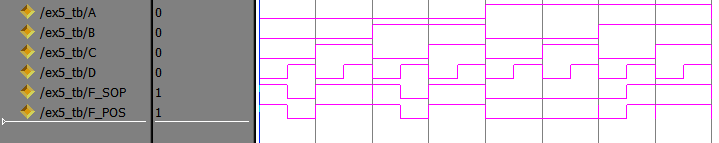
\includegraphics[width=\textwidth]{lab5_procedure}
	\caption{Circuit simulation using the test bench}
	\label{fig:simulation}
\end{figure}

Figure \ref{fig:simulation} shows all of the input combinations of the 4-input function function. The two outputs generate the same waveform because they are different implementations of the same function.

\section*{Conclusion}

The purpose of this exercise was to analyze the efficiency of min-term (SOP) and max-term (POS) function implementation. An arbitrary function was provided. Two Karnaugh maps were generated and used to extract the SOP and POS expressions. These expressions were then implemented in a circuit in Quartus II and simulated in Modelsim. The cheaper circuit was then constructed on a breadboard. This experiment was successul in obtaining the correct output set as provided by the function from the breadboard and the simulation.

\pagebreak

\section*{Questions}

\begin{enumerate}
  \item Design a two level NAND-NAND implementation of $F_{SOP}$.
  
\begin{figure}[htbp]
	\centering
	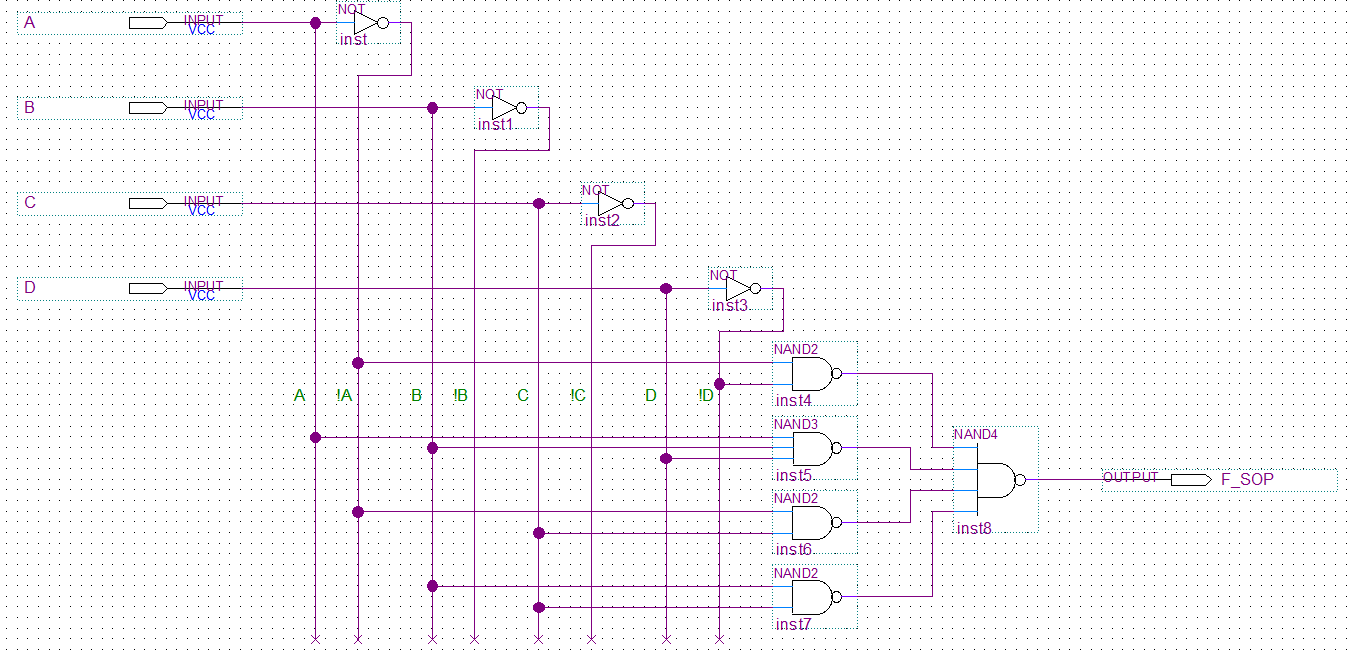
\includegraphics[height=7.5cm]{nand-nand}
	\caption{Two level NAND-NAND implementation of $F_{SOP}$}
	\label{fig:nand-nand}
\end{figure}

  \item Design a two level NOR-NOR implementation of $F_{POS}$.
  
\begin{figure}[htbp]
	\centering
	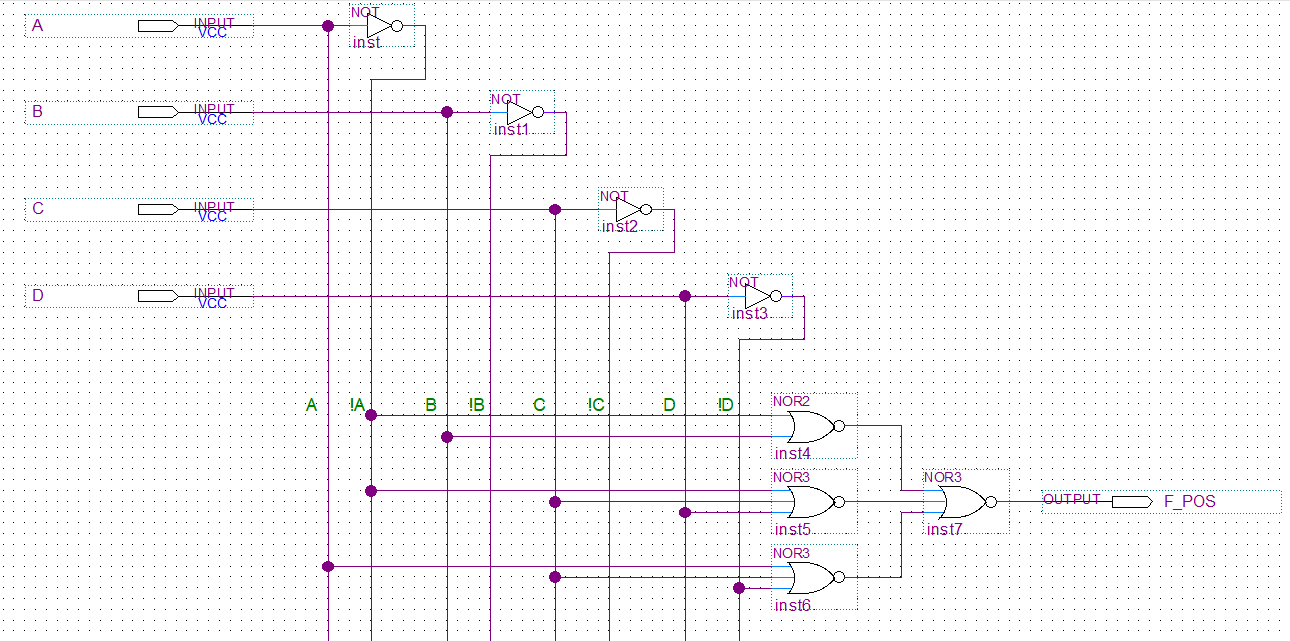
\includegraphics[height=7.5cm]{nor-nor}
	\caption{Two level NOR-NOR implementation of $F_{POS}$}
	\label{fig:nor-nor}
\end{figure}
\end{enumerate}

\end{document}
